\documentclass{sigchi}

% Load basic packages
\usepackage{balance}  % to better equalize the last page
\usepackage{graphics} % for EPS, load graphicx instead 
\usepackage{mathptmx}
\usepackage[pdftex]{hyperref}
\usepackage{color}
\usepackage{booktabs}
\usepackage{textcomp}
\usepackage{microtype} % Improved Tracking and Kerning
\usepackage{ccicons}  % Cite your images correctly!
\usepackage{multicol}
\usepackage{color} 
\newcommand{\hl}[1]{\colorbox{yellow}{#1}}
\usepackage{xspace}
\usepackage{algorithm} 
\usepackage{algpseudocode} 
\usepackage{subcaption}
\usepackage{booktabs}
\def\algname{SPRING\xspace}
\DeclareMathOperator*{\argmin}{argmin}
\DeclareMathOperator*{\argmax}{argmax}

\floatname{algorithm}{Procedure}
\renewcommand{\algorithmicrequire}{\textbf{Input:}}
\renewcommand{\algorithmicensure}{\textbf{Output:}}


\usepackage{tikz}
\usetikzlibrary{decorations.pathreplacing,calc}
\newcommand{\tikzmark}[1]{\tikz[overlay,remember picture] \node (#1) {};}
\newcommand*{\AddNote}[4]{%
    \begin{tikzpicture}[overlay, remember picture]
        \draw [decoration={brace,amplitude=0.2em},decorate, thick, darkgray]
            ($(#3)!(#1.north)!($(#3)-(0,1)$)$) --  
            ($(#3)!(#2.south)!($(#3)-(0,1)$)$)
                node [align=center, text width=2.5cm, pos=0.5, anchor=west] {#4};
    \end{tikzpicture}
}%


% Paper metadata (use plain text, for PDF inclusion and later
% re-using, if desired).  Use \emtpyauthor when submitting for review
% so you remain anonymous.
\def\plaintitle{A Data-Driven Approach for Inferring Student Proficiency from Game Activity Logs  }
\def\plainauthor{Mohammad H. Falakmasir, Jos\'{e} P. Gonz\'{a}lez-Brenes, Geoffrey J. Gordon, Kristen E. DiCerbo}
\def\emptyauthor{}
\def\plainkeywords{Authors' choice; of terms; separated; by
  semicolons; include commas, within terms only; required.}
\def\plaingeneralterms{Documentation, Standardization}


% llt: Define a global style for URLs, rather that the default one
\makeatletter
\def\url@leostyle{%
  \@ifundefined{selectfont}{
    \def\UrlFont{\sf}
  }{
    \def\UrlFont{\small\bf\ttfamily}
  }}
\makeatother
\urlstyle{leo}

% To make various LaTeX processors do the right thing with page size.
\def\pprw{8.5in}
\def\pprh{11in}
\special{papersize=\pprw,\pprh}
\setlength{\paperwidth}{\pprw}
\setlength{\paperheight}{\pprh}
\setlength{\pdfpagewidth}{\pprw}
\setlength{\pdfpageheight}{\pprh}

% Make sure hyperref comes last of your loaded packages, to give it a
% fighting chance of not being over-written, since its job is to
% redefine many LaTeX commands.
\definecolor{linkColor}{RGB}{6,125,233}
\hypersetup{%
  pdftitle={\plaintitle},
% Use \plainauthor for final version.
%  pdfauthor={\plainauthor},
  pdfauthor={\emptyauthor},
  pdfkeywords={\plainkeywords},
  bookmarksnumbered,
  pdfstartview={FitH},
  colorlinks,
  citecolor=black,
  filecolor=black,
  linkcolor=black,
  urlcolor=linkColor,
  breaklinks=true,
}

% create a shortcut to typeset table headings
% \newcommand\tabhead[1]{\small\textbf{#1}}

% End of preamble. Here it comes the document.
\begin{document}

\title{\plaintitle}

\numberofauthors{4}
\author
{%
  \alignauthor{\mbox{\hspace{-1.85em}Mohammad H. Falakmasir$^{\star, \#} $\;\;\; Jos\'{e} P. Gonz\'{a}lez-Brenes$^\star$ \;\;\; Geoffrey J. Gordon$^\S$ \;\;\; Kristen E. DiCerbo$^\star$}\\
    \affaddr{$^\star$School Research}\\
    \affaddr{Pearson}\\
    \email{\{jose.gonzalez-brenes, kristen.dicerbo\}@pearson.com }\\
    }
  \alignauthor{\vphantom{Mohamamad Jose}
    \affaddr{$^\#$Intelligent Systems Program} \\
    \affaddr{University of Pittsburgh}\\
    \email{falakmasir@pitt.edu}\\
  }
  \alignauthor{\vphantom{Mohamamad Jose}
  	\affaddr{$^\S$Machine Learning}\\
	\affaddr{Carnegie Mellon University} 
  	\email{ggordon@cs.cmu.edu}\\
  }
}

  
\maketitle

\begin{abstract}
		Traditional assessments are important in education because they allow collecting evidence about student progress. 
		Unfortunately, they can be very tedious to their stakeholders.
		In contrast, invisible assessment  unobtrusively gathers  performance data from students' daily activities to make inference about student relevant competency.
We present a novel data analysis pipeline, {Student Profficiency Inferrer from Game data} (\algname), that allows modeling  game playing behavior in educational games.
Unlike prior work, \algname is a fully data-driven method that does not require costly domain knowledge engineering.
We validate our method using data collected from students playing 11 educational mini-games.
Our results suggest that  \algname is accurate to predict Math assessments ($R^2$ =0.55 , Spearman $\rho$=0.82).
%We provide insights in how to use \algname to understand student exploration habits, misconceptions, and how to improve the game design based on their playing strategies.
\end{abstract}

\category{K.3.1}{Computer Uses in Education.}
{}
\keywords{Educational Games, Student Modeling, Stealth Assessment}

\section{Introduction}
Educational assessments are important because they collect evidence about about  whether  the teaching goals are being met.
Unfortunately, the process of  administering assessments is usually disconnected to the learning environment, and  it is often  disruptive to the classroom. 
In many developed countries, students now find themselves spending increasing amounts of time preparing and taking tests instead of learning~\cite{hofman2015rebalancing}.
For example, a  survey of the current state of testing in America revealed that students are taking an average of 113 standardized tests between pre-K and highschool~\cite{lazarin2014testing}. 
For these reasons, it is not surprising that the recent political climate and the general population have been weighing in on the question of whether students are being tested too much~\cite{lazarin2014testing}.


According to Evidence Centered Design (ECD)~\cite{mislevy2012design}, the goal of assessment is to characterize the strength of evidence regarding claims one wants to make about individuals or groups.
Therefore, the assessment process involves identifying, organizing, or creating activities for students so we may observe that evidence.
An interesting alternative to traditional summative assessment is invisible (or stealth) assessment~\cite{shute2013stealth},
where the evidence is gathered from leaners unobtrusively from the digital interactions of their ongoing activities.
This data is used  to understand claims regarding what students know and what they can do \cite{shute2009melding}.
Stealth assessment is also intended to reduce or eliminate test anxiety, while not sacrificing validity and reliability \cite{shute2008you}.



A promising opportunity for invisible assessment is using log data collected from educational games.
Unfortunately, engineering a system that parses logs is costly and time-consuming.
For example, prior work~\cite{shute2013stealth, shute2009melding} has relied extensively on subject matter expertise to define a student model in form of a  Bayesian Network to build both the competency model, and to extract features of the performance data.

Our motivation is that invisible assessment from game data may become more accurate and cheaper to implement if the domain knowledge engineering could be automated by a data-driven process.
Game data is often logged  with what we call a \textit{slot and filler} structure.
In Table~\ref{tbl:log_example}, we show a simplified example of a real educational game log that uses slot and filler structure.
The slots are discrete sets of events that are initiated by the leaner.
Each slot may accept zero to multiple fillers. 
Each filler represents a value of a property of the slot event.
For example, a \texttt{Move Object} event  that represents the learner moved an object in the screen, may have an $x$ and $y$ coordinates as fillers to represent the target position in two-dimensional space.

\begin{table}[tbh]
	\begin{tabular}{@{}llll@{}}
		\toprule
		\textbf{Id}             & \textbf{User Id} & \textbf{Event Name} & \textbf{Event Data}        \\ \midrule
		1                       & ABC              & Game Start          & \{ \}                        \\
		2                       & ABC              & Move Object         & \{X:363,Y:82\} \\
		3                       & ABC              & Move Object         & \{X:361,Y:54\} \\
		4                       & ABC              & Open Toolbox        & \{\}        \\
		4                       & ABC              & Activate Tool        & \{tool:gluumi\}        \\
		5                       & ABC              & Use Gluumi        & \{sizeGluedTo:8,sizeNew:9\} \\        
		\multicolumn{1}{c}{...} &                  &                     &                            \\ \bottomrule
	\end{tabular}
	\caption{An example fragment of a log from an educational game. \label{tbl:log_example}}
\end{table}
\hl{I renamed X and Y for simplicity, hope that's ok} 
% http://www.tablesgenerator.com/#

Conventional machine learning algorithms cannot input slot and filler data, as they  work in  structures called \textit{feature vectors} or \textit{sequences}.
Prior work~\cite{sequences} provides a   review of  the difference between feature vectors and sequences.
A feature vector representation requires mapping an observation onto a fixed number of features.
It is not trivial to map sequences of student actions that can be of an arbitrary length into a feature vector that needs to be of a predetermined dimension.
Traditional feature vector classifiers,  like logistic regression or decision trees,  that are used in off-the-shelf data mining packages, such as Weka \cite{hall2009weka}, cannot  use slot and filler data as input. 
In contrast, machine learning algorithm that allow sequential representations, like Hidden Markov Models (HMM), require a parametric model with the same number of dimensions for all of the observations.
This does not occur in slot and filler structures.
For example,  in Table~\ref{tbl:log_example}, the \texttt{Move Object} slot requires \texttt{x} and \texttt{y} fillers, while the \texttt{Use Gluumi} slot requires \texttt{size} fillers.

In this paper, we propose \textit{Student PRofficiency INferrer from Game data} (SPRING), a novel data analysis pipeline that models game playing behavior.
\algname allows modeling raw data in slot and filler structure.
We demonstrate our approach on real student game playing data.
Our experiments suggest that \algname can be used to predict student proficiency  without costly domain expertise.

\section{SPRING Framework}

\algname is designed in a way that can capture sequential decision making process of students in a way that is representative of their mastery with minimum reliance on expert knowledge. Our data analysis pipeline receives raw data of student interactions with the different levels of educational game in slot and filler format along with their post-test results and creates a regression model for predicts the post-test score. 
Algorithm~\ref{alg:spring} describes the three main steps of our pipeline: discretization,  sequence modeling, and regression.
\hl{Explain briefly in words what the whole thing does}.
We now explain the different steps in detail.

\begin{algorithm}
\begin{algorithmic}[1]
\Require: A log file $\mathbf{L_{g,s}}$ of slot-filler structure for each game $g$ and student $s$, a test $y_s$ for each student
\State  $\langle \mathbf{L'_{g,s}} , c_s \rangle \leftarrow$  Cluster\_students($\mathbf{L_{g,s}}, y_s$) \tikzmark{disctop}\tikzmark{right}\tikzmark{secright}
\State $\mathbf{x_{g,s}} \leftarrow$  Discretize($\mathbf{L'_{g,s}}$) \tikzmark{discbot}
\For {each  game $g$}  \tikzmark{sectop}
\For{each cluster  $c_s$}
\State  $\theta_{g,c_s} \leftarrow$  Learn\_HMM($ \mathbf{x_{g,s}} $) 
\EndFor
\EndFor \tikzmark{secbot}
\State Prediction $y_s$  from $x_{g,s}, \theta_{g, c_s}$ \tikzmark{regtop}
\tikzmark{regbot}
\end{algorithmic}
\AddNote{disctop}{discbot}{right}{Discretization}
\AddNote{sectop}{secbot}{right}{Sequence Modeling}
\AddNote{regtop}{regbot}{right}{Regression}
\caption{The SPRING algorithm\label{alg:spring}}
\end{algorithm}



\subsection{Discretization}
\hl{Each section should refer to line numbers in the algorithm}
\hl{Make sure the notation is consistent between algorithm and steps}
The discretization inputs time-ordered slot and fillers events and converts them into sequences of discrete observations.
For this, we use a clustering algorithm called DBSCAN~\cite{ester1996density} on the fillers. 
We use DBSCAN because it % student interaction with our educational game 
%was dominated by moving objects in a 2 dimensional space.
%We tried different unsupervised and non-parametric methods, however, we ended up using DBSCAN because it 
can find arbitrarily shaped clusters and does not require one to specify the number of clusters in the data a-priori. 
It is also robust to outliers which in our case can be interpreted as noisy movements that are not representative of learning competency. 
We considered outliers as a separate cluster. \hl{?? ... explain}

Figure~\ref{fig:figurecluster} shows an example of using clustering to discretize \texttt{Move Object} slots, that have $x$ and $y$ coordinates as fillers.
Figure~\ref{fig:screenshot} shows a screenshot of an educational game where students have to move ice cubes from the mountain top onto some designated areas.
Figure~\ref{fig:figurecluster} shows a scatterplot of \hl{write... you need to explain this}.
We colored the points according to the DBSCAN clustering.
In this example, we have three clusters,  cluster one and two represent the \hl{the most common positions}, and cluster three are the the outliers.

\begin{figure}[t]
 \centering
\begin{subfigure}{.5\textwidth}
	\centering
	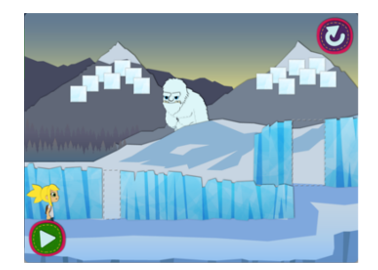
\includegraphics[width=0.9\columnwidth]{figures/glacier_screenshot.png}
	\caption{\hl{write} \label{fig:screenshot}}
\end{subfigure}
\begin{subfigure}{.5\textwidth}
	\centering
	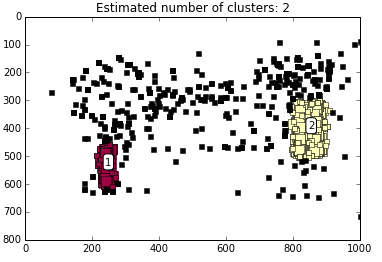
\includegraphics[width=0.9\columnwidth]{figures/glacier_positions.png}
	\caption{\hl{write} \label{fig:clustering}}
\end{subfigure}
\caption{The clusters detected for game level 2, \textit {None Shall Pass!}, using DBSCAN method. We transform each movement action into corresponding cluster id during the discretization step.\label{fig:figurecluster}}
\end{figure}

After running DBSCAN on the filler dimensions, we trained a K-Nearest Neighbor Classifier on the cluster labels in order to convert the sequence of slot and filler observations into a two dimensional array of multinomial observations \hl{why?? DBSCAN already does this.  You need to document why you did this. explain each step and rationale so people can understand the intelligence of the approach. if not it will sound arbitrary}.
We also used this classifier to transform any unseen sequence of interactions for our empirical evaluation phase. The details of the discretization phase is demonstrated in Procedure~\ref{alg:discretize}.
\hl{Show an example input (slot-filler), and an example output (discrete sequence) to help illustrate the point}

\begin{algorithm}
	\begin{algorithmic}
		\Procedure{Discretize}{S}
		\State{A = empty dictionary of slots and possible fillers}
		\For{each sequence s in S }
		\For{each action a in s}
		\If{a.filler $\neq \varnothing$}
		\State{A[a.slot].append(a.filler)}
		\EndIf
		\EndFor
		\EndFor
		\State
		\For{each slot and fillers tuple in A}
		\State{clustersIDs = DBSCAN(a.fillers)}
		\State{C[a.slot] = K-NN classifier on fillers and clusterIDs}
		\EndFor
		\State
		\State{D = [][]\textit{ --2D array of multinomial observations}}
		\For{each sequence s in S}
		\State{P[i] = s.post-test}
		\For{each action a in s}
		\State{D[i,j] = C[a.slot].predict(filler)}
		\EndFor
		\EndFor
		\State \Return{D}
		\EndProcedure
		
	\end{algorithmic}
	\caption{The Discretization Step of \algname \label{alg:discretize}}
\end{algorithm}



\subsection{Sequence Modeling}
In the modeling phase, we hypothesized that high- and low-performing students have similar usage patterns that are representative of their sequential decision-making process. 
Our model should be able to successfully capture this difference across different game levels and use it to predict post-test scores.
Hidden Markov Models are good candidate for the task of unsupervised analysis of sequential data.
Given the sequence of student actions, we aim to infer meaningful sequence of (latent) states, which describe the process that generated the actions, along with statistical patterns that can describe and distinguish those states.
Since a large portion of student interactions are based on the logic of the game, we had no idea about the number of states and what they mean.
As a result, we used the Hierarchical Diriclet Process HMM (HDP-HMM) \cite{fox2008hdp}, which is allows state spaces of unknown size to be learned from data. 
HDP-HMM defines a \textit{hierarchical Dirichlet process} prior on transition matrices over countably infinite state spaces and is able to make a principled choice of how many states it needs based on the complexity of its training data. 
For details on training methods please refer to \cite{fox2008hdp}.

We used the output of the discretization step (2D array of multinomial observations) and trained two HDP-HMMs, one for high-performing and the other for low-performing students in each game level. The two models can be considered as a stochastic representation of the sequence of actions and we can use them to infer the likelihood of any arbitrary sequence as a feature for the regression step.

\hl{For simplicity, here we assume only two clusters for students being in either  high or low performing groups.}
\hl{Talk about Forward backward algorithm, and how you calculate theta!!!}

\subsection{Regression}

%In this phase, we created a linear regression model using the likelihoods extracted from the previous phase. 
For each student $s$  in each game level $g$, we calculate the difference ($d_{s,g}$) of the likelihood of   belonging to high performing group minus the likelihood of of belonging to the low performing group.
We calculate this likelihood by estimating the Forward-Backward probabilities  on each student sequence sequence of actions  based on the two HMMs parameter we estimated (whether the student is in the high performing group or in the low performing group):
\begin{equation}
d_{s,g} = \theta_{g, \text{high}} - \theta_{g, \text{low}}
\end{equation}

We use  a linear regression model for predicting the post-test scores:


\begin{equation}
\hat {y_s}(\beta) =   \sum_g \beta_g \cdot d_{s,g}  + \beta_0
\end{equation}

Here, $\beta_0$ is just an intercept for the  model.  
We can optimize the parameters using \hl{what algorithm?}.
We experimented with different regularization methods, but only report \hl{LASSO ??} \hl{cite} as it worked best in our preliminary comparisons:
\begin{equation}
\beta^* = \argmin_\beta || y_s - \hat{y_s}(\beta)  ||_2 + \lambda \cdot || \beta ||_1
\end{equation}


\section{Empirical Evaluation}

\subsection{Game Environment}
\textit {Alice in AreaLand} is an educational game developed for research purposes. It focuses on teaching and assessing geometric measurement, specifically the understanding of area, among 6th grade students. The game targets three main stages in the development of area: 1) area unit iteration, 2) use of unit squares to measure area, and 3) use of composites to measure area. The current version has 11 game levels. A simple student scenario involves covering a 2D area with smaller unit squares placed end-to-end in non-overlapping fashion, combining the single squares into rows or columns, and then determining the number of rows or columns needed. Figure~\ref{fig:figurekracken} shows a screenshot of one game level.

\begin{figure}
	\centering
	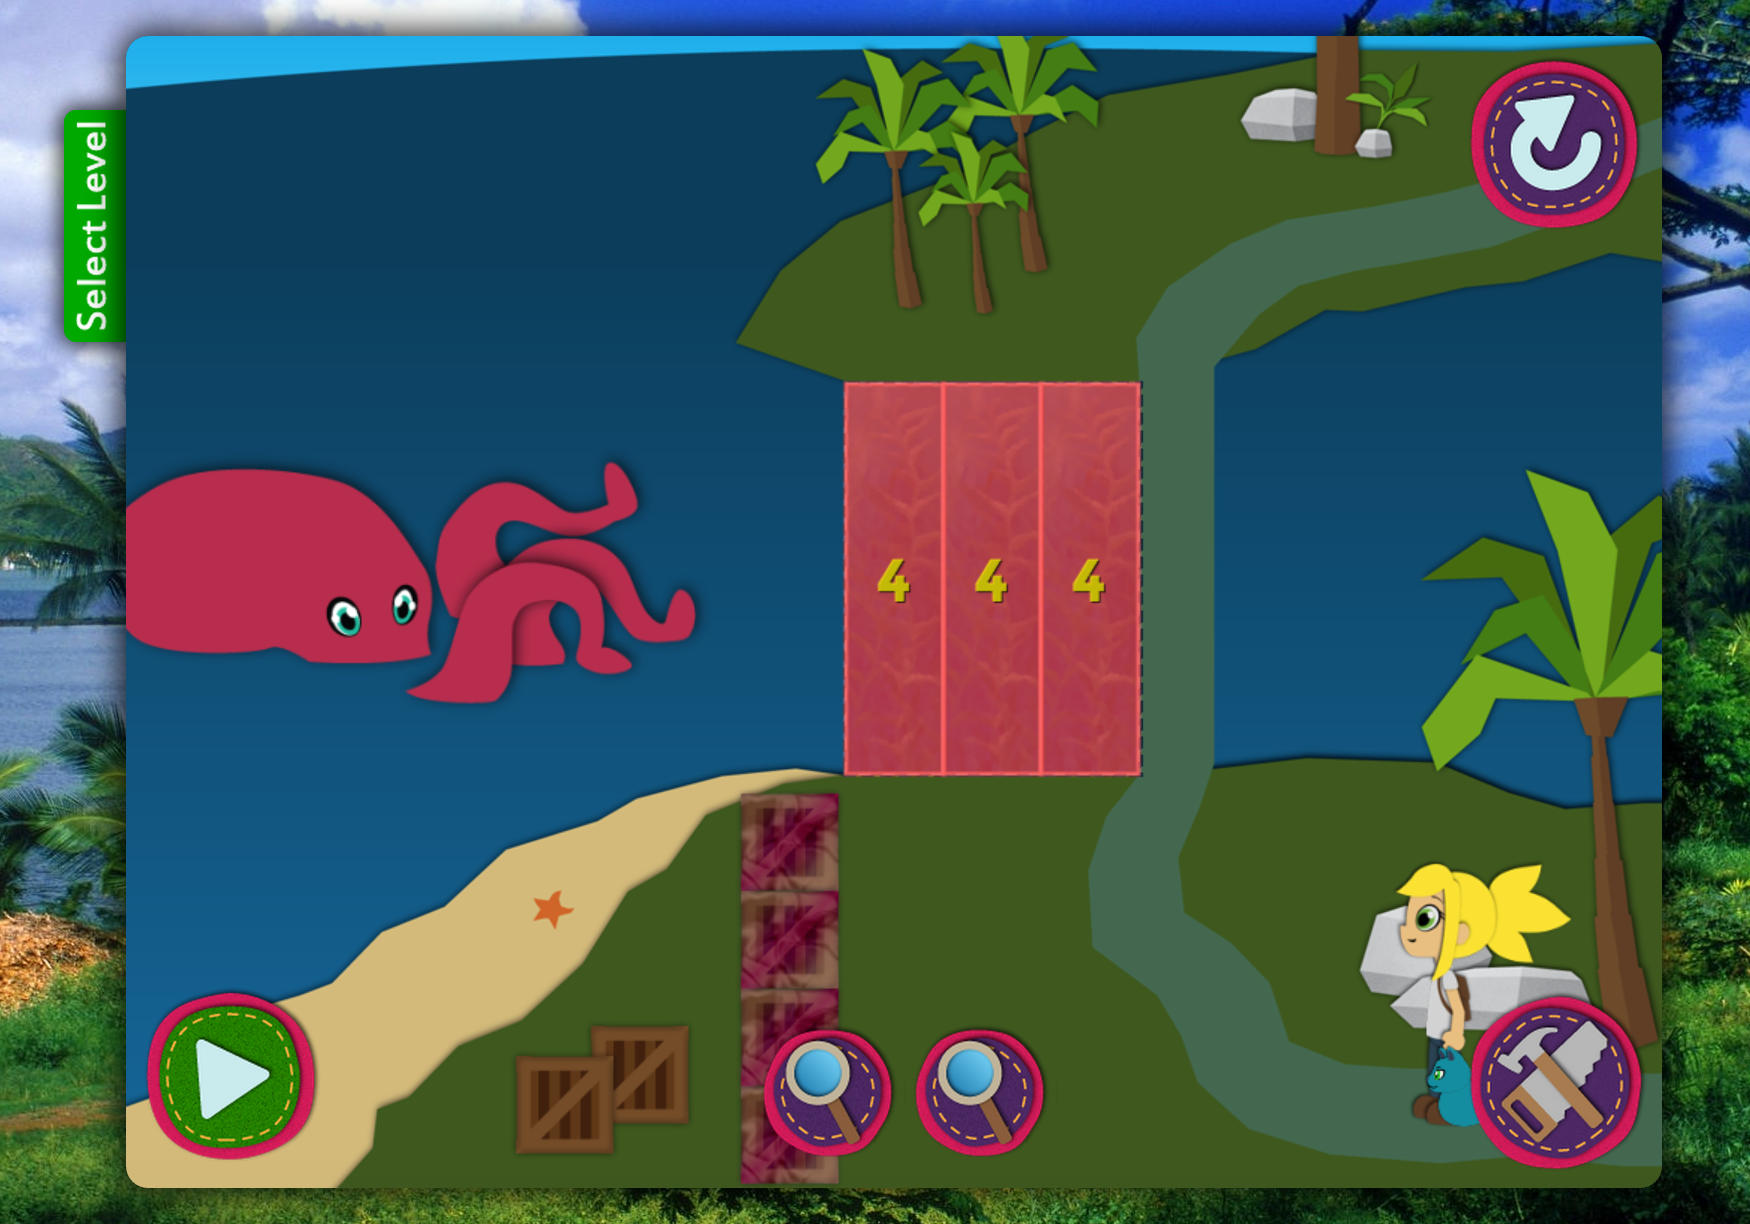
\includegraphics[width=0.9\columnwidth]{figures/kracken}
	\caption{A screenshot of hint provided in game level 11, \textit {You Kraken Me Up!}, in \textit {Alice in AreaLand}. Students should combine four squares into a column and create three copies of the column to cover the designated area and prevent the octopus from attacking \textit {Alice} while she crosses the bridge.}~\label{fig:figurekracken}
\end{figure}

Throughout the game,  \textit {Alice} is accompanied by \textit {Flat Cat} -- an assistant character who provides feedback and scaffolding to the player in the beginning of each game level and upon request when students push a hint button (represented by two magnifiers at the bottom center of Figure ~\ref{fig:figurekracken}). Earlier game levels are designed for students to learn about area unit iteration and usually require them to cover a number of predefined areas with unit squares (not necessarily in a non-overlapping fashion). By advancing through game levels, students are presented with three tools: \textit {Gluumi} for combining unit squares by gluing them together; \textit {Multy}, for making copies of different objects; and \textit {Esploda} for breaking compound shapes into single units.  There is no limit for completing a game level regarding time or number of actions students may execute. The students press the \textit {Go Alice} button (bottom left corner of Figure~\ref{fig:figurekracken}) if they deem their performance to be satisfactory for \textit {Alice} to proceed. Based on the covered area and the arrangement of the tiles, they either advance to the next level or receive a feedback and stay in the same level.

\subsection{Dataset} 
Our dataset consists of time-stamped interactions of 129 students in 11 game levels. 
For 77 students, we also have post-test scores from a paper-based exam with 20 questions in the 3 skills of geometric measurement.
In total, there are 88,458 events recorded in the dataset from 1,510 game sessions, meaning that student tried some of the game levels for multiple times.
Based on the ECD framework, beginning levels only involve area unit iteration skill and the other skills and related features are gradually added to the later game levels.
Figure \ref{fig:frequency} shows the frequency of different events in each game level. As depicted in Figure \ref{fig:frequency}, the student interactions with the system in all game levels is dominated by movements.

\begin{figure}
	\centering
	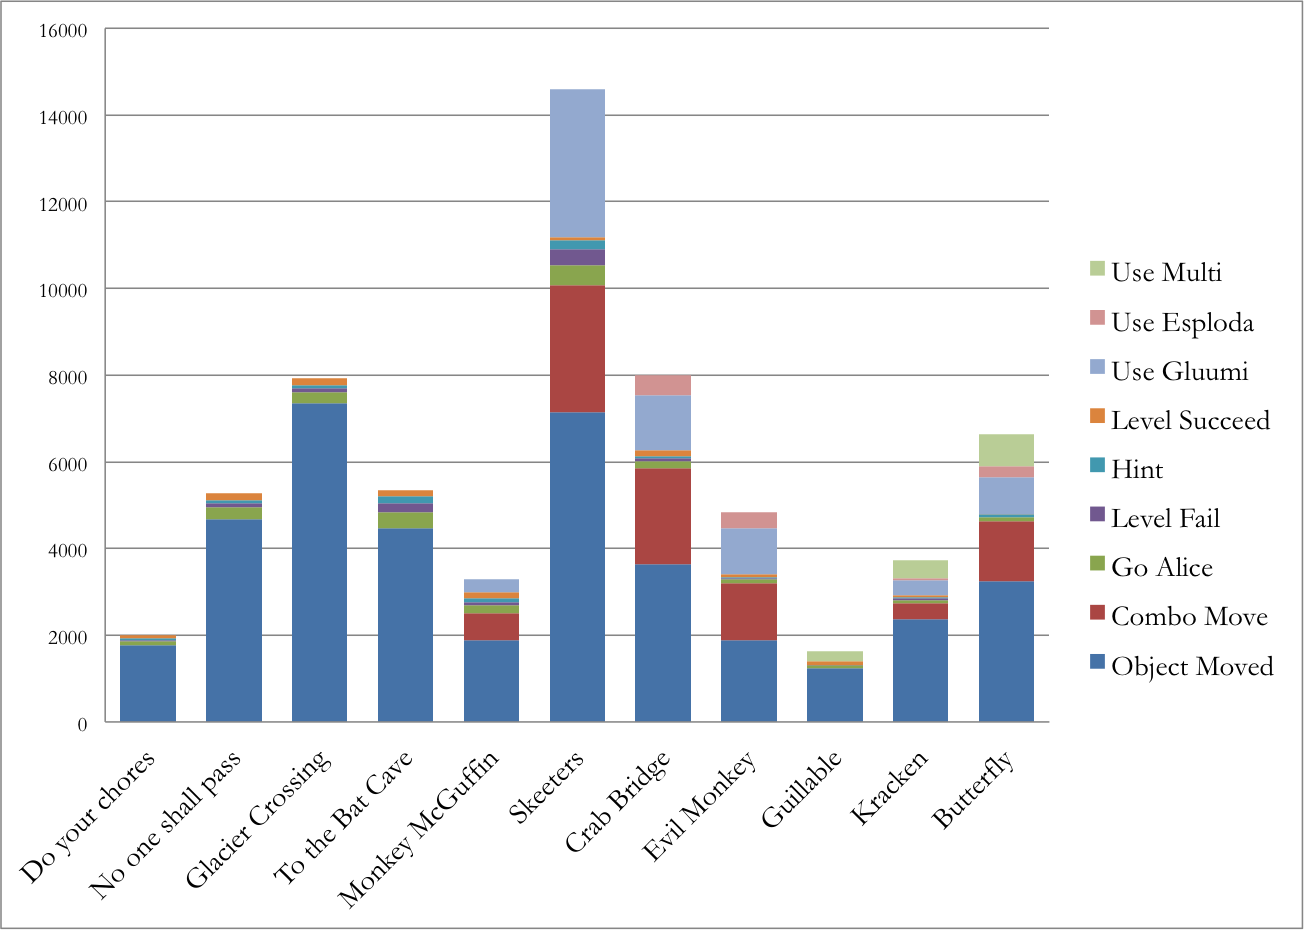
\includegraphics[width=0.9\columnwidth]{figures/frequency}
	\caption{Frequency of Events in Each Game Level}~\label{fig:frequency}
\end{figure}

We only used the trajectories of the students who participated in the post-test.
In the case of multiple attempts in a game level, we only considered the trajectory from the first attempt.
Figure \ref{fig:boxplot} shows the boxplot of sequence length in each game level.

\begin{figure}
	\centering
	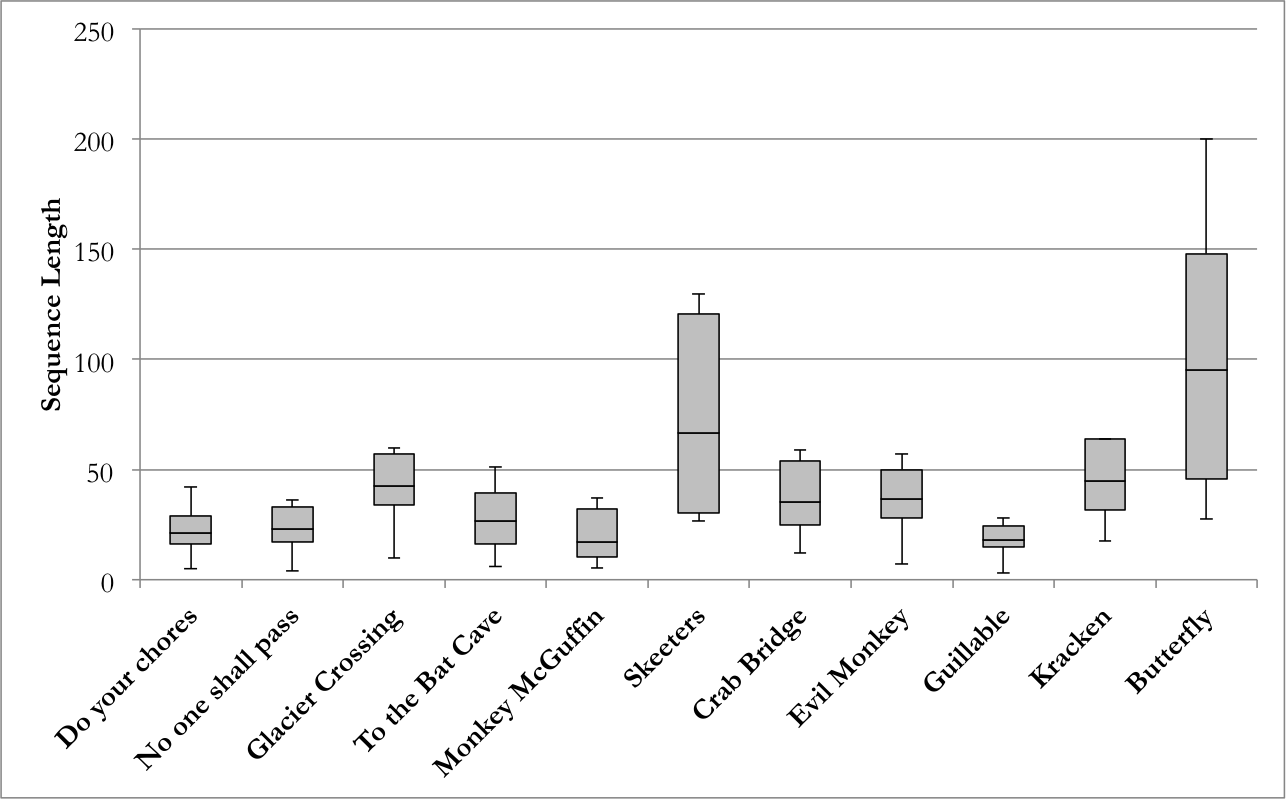
\includegraphics[width=0.9\columnwidth]{figures/boxplot}
	\caption{Boxplot of Sequence Length in Each Game Level}~\label{fig:boxplot}
\end{figure}

\subsection{Experimental Setup}
First we divide students into two groups, one (\%80) for training and development purposes and the other (\%20) for test and verification.
In the synthesis phase, we transform log data of different nature (eg. movements, use of the tools, requests for hints) in each game level to observable values that can be used as evidence for learning.
In the modeling phase, we use the observations to train two Hidden Markov Model (HMM)s that capture the sequence of actions for high- and low-performing students.
In the aggregation phase, we uses the likelihood of students' sequence of action in order to build a regression model that is predictive of the post-test results.
Finally, we test the regression model on the held-out set (\%20) and report the results.


\subsection{Results}
In order to evaluate our regression model we decided to compare its performance agains two baselines: 1) A regression model that uses success and failure of students in each game level as feature \hl{Write equation}and 2) A regression model that uses the sequence lengths in each game level \hl{Write equation}. 
Our model was able to significantly outperform both baselines regarding to mean absolute error and root mean squared error. 
Moreover, the $R^2$ correlation and Spearman $\rho$ of our predicted values with the true values was much higher than both baselines. Table \ref{tab:results} shows the results.


\begin{table}[tbh]
	\centering
	\begin{tabular}{@{}lllll@{}}
		\toprule
		\begin{tabular}[c]{@{}l@{}}\textbf{Predictive Features}\end{tabular}            & \begin{tabular}[c]{@{}l@{}}\textbf{$R^2$}\end{tabular} & \begin{tabular}[c]{@{}l@{}}\textbf{$\rho$}\end{tabular} & \begin{tabular}[c]{@{}l@{}}\textbf{MAE}\end{tabular} & \textbf{RMSE}\\ \midrule
		\begin{tabular}[c]{@{}l@{}}Sequence Length (Normal)\end{tabular} & 0.06                                                     & 0.79                                                 & 3.24                                                          & 4.15 \\
		Success / Failure                                                      & 0.01                                                     & 0.63                                                 & 3.22                                                          & 4.14 \\
		\algname                                                       & 0.55                                                     & 0.82                                                 & 2.84                                                          & 3.35 \\ \bottomrule
	\end{tabular}
	\caption{The results of predicting post-test scores using three different feature sets}~\label{tab:results}	
\end{table}

	\hl{Show residual plot}
	\hl{Show confidence intervals}
	
\subsection{Discussion}
Figure~\ref{fig:highvslow} shows the difference between two HMMs learned for one of the game levels.

\begin{figure}
	\centering
	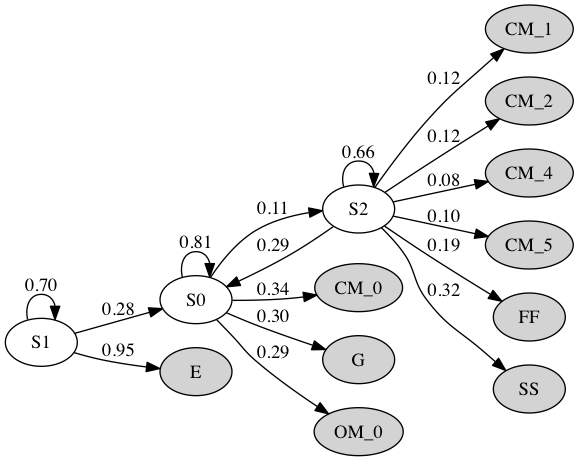
\includegraphics[width=0.9\columnwidth]{figures/high}
	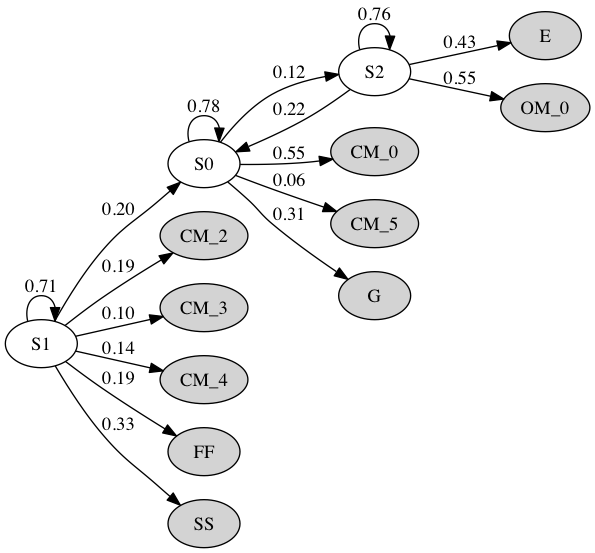
\includegraphics[width=0.9\columnwidth]{figures/low}
	\caption{Two Hidden Markov Models learned from data in one of the game levels. The top HMM represents the high-performing students and the bottom one represents the low-performing ones.}~\label{fig:highvslow}
\end{figure}


\section{Relation to Prior Work}
In order to deal with such highly unstructured data, researchers often use carefully designed network structures (such as Bayesian Networks \cite{albrecht1998bayesian,shute2013stealth}) or game-specific heuristics and benchmarks generated by experts playing the game \cite{mandel2014offline,tastan2011learning}. However, this approach is extremely labor intensive and might fail to capture meaningful patterns in student exploratory habits within the game. Given these limitations, data-driven analysis of student interactions provides a powerful alternative that facilitates the discussions around what does and does not work in a particular educational game.

The potential of computer games for educational purposes has been of interest since nearly the beginning of videogames. Unlike video games, which focus on creating an entertaining experience for the user, educational games require principles and strategies that engage students while maximizing their learning gain. Therefore, data-driven analysis of student behavior is crucial to better understand the learning process and improve the tools in the future.

There have been numerous attempts among the educational research community to develop analytic methods and build predictive models based on the data from educational games. \textit{Newton's Playground} is an ECD based educational game with 74 problems that designed to teach qualitative physics to students in eighth- and ninth-grade. Students have to guide a green ball to a red ball by creating simple machines. 
Everything obeys the basic rules of physics relating to gravity and Newton’s three laws of motion. 
Shute et al. \cite{shute2013stealth} studied the effect of ECD design on student learning and found that students who played the game in a 4 hour session, showed significant improved in their qualitative, conceptual physics understanding.

\textit {Rumble Blocks}  is another educational game designed to teach basic concepts of structural stability and balance to children in grades K-3 (ages 5-8 years old). Harpstead et al. \cite{harpstead2014using}, studied the alignment of game to its target learning goals by examining whether student solutions follows the targeted principals. They employ clustering techniques on the individual solutions created by actual students and use principle-relevant metric (PRM) to measure how closely the representative solution embodies a specific targeted principle. The results demonstrated a misalignment between the feedback provided to students and the targeted knowledge.

\textit {Battleship Numberline} is another educational game for understanding fraction using number line estimation. Students attempt to explode target ships and submarines by estimating numbers on a number line. Lomas et al. \cite{lomas2013optimizing} performed a large-scale online experiment in order to study the effect of challenge on player motivation and learning. They presented different configurations of the game for different groups of students and used a combination of time spent and challenges attempted as a measure of engagement and the average success rate of each design configuration as a measure of challenge. The results showed a linear correlation between challenge (difficulty) and engagement, meaning the easier the game, the longer students played.

\textit {Refraction} is another educational game for learning about fractions by splitting laser beams into fractional amounts to target spaceships by avoiding asteroids. Liu et al. \cite{liu2013predicting}, created an ensemble algorithm that combines elements of Markov models, player heuristic search, and collaborative filtering techniques with state-space clustering in order to predict player movements on last game-level based on the history of movements in previous game levels. Lee et al. \cite{lee2014learning} extended the former framework by building state-action graph and using feature selection techniques to reduce the number of features for each state. To ensure extensibility, they also tested the framework on another game \textit {DragonBox} and reported improvement over a Markov predictor.

\section{Conclusion}
\hl{Limitation, we don't compare to Valerie Schultz}

\hl{Limitation, we don't control for game ability like Valrerie does}

\hl{Limitation, we only used data from Alice in wonderland}

\hl{Method is accuaate}


\bibliographystyle{SIGCHI-Reference-Format}
\bibliography{references}

\end{document}
